% !Mode:: "TeX:UTF-8"
% !TEX program  = xelatex
\documentclass[a4paper]{article}
\usepackage{amsmath}
\usepackage{amssymb}
\usepackage{ctex}
\usepackage{graphicx}
%\usepackage{braket}
\usepackage[european]{circuitikz}
\usepackage{multirow}
\usepackage{geometry}
\usepackage{float}
\geometry{left=2.5cm,right=2.5cm,bottom=2.5cm,top=2.5cm}
\title{物理化学实验: 纳米$TiO_{2}$光催化降解甲基橙}
\author{薛明怡\quad 151250177\quad 化学化工学院}
\date{\today}
\begin{document}
\maketitle
%%\tableofcontents
%%\bibliographystyle{unsrt}
\section{实验目的}
\begin{enumerate}
\item 测定纳米$TiO_{2}$对甲基橙光催化降解反应的催化活性.
\item 掌握一种光催化反应的实验方法.
\end{enumerate}
\section{实验原理}
\subsection{$TiO_{2}$纳米粒子}
$TiO_{2}$主要有如下两种晶型, 左图为金红石型, 右图为锐钛矿型. 
其中锐钛矿型具有较高的光催化活性, 研究和应用中多采用锐钛矿$TiO_{2}$.
\begin{figure}[H]
	\centering
	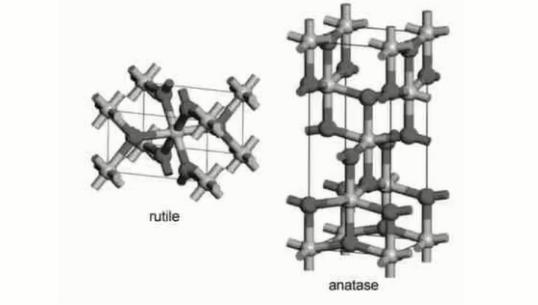
\includegraphics[width = 0.5\paperwidth]{fig/crystalline.png}
	\caption{二氧化钛的两种晶型}
\end{figure}
\par
在光照的作用下, $TiO_{2}$价带(valance band, VB)电子跃迁至导带(conduction band, CB),
产生一定的激发态电子$e^{-}$和电子空位$h^{+}$, 其中一部分在催化剂内部复合回到
基态, 另一部分则转移至催化剂的表面. 激发态电子$e^{-}$和电子空位$h^{+}$在催化剂
表面也会复合, 剩余的一部分则通过与系统中处于催化剂周围的分子或离子发生电子交换而
回到基态, 即发生化学反应, 整个过程就是光催化反应, 图示如下.
\begin{figure}[H]
	\centering
	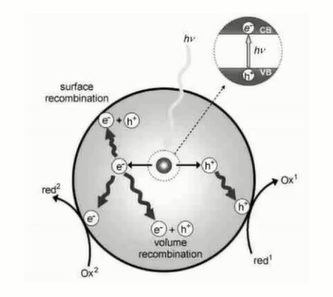
\includegraphics[width = 0.4\paperwidth]{fig/principle.png}
	\caption{光催化反应原理}
\end{figure}
\par
\subsection{光催化反应}
光催化反应是光化学反应的一种. 光化学反应有别于热化学反应, 在恒温恒压下可以使一些系统的Gibbs自由能增加, 
例如光合作用, 光解水制氢等. 但如果把辐射光源切断, 则该反应仍旧向Gibbs自由能减少的方向进行, 力图
回复原来的状态. \par
热化学反应活化能源于分子碰撞, 而光化学反应的活化能源于光子的能量(光化学反应的活化能通常为$30kJ\cdot mol^{-1}$
左右, 小于一般热化学反应的活化能). 热化学反应的反应速率受温度影响大, 而光化学反应的温度系数小. \par 

\subsection{多相催化反应}
对于多相催化反应而言, 反应物在催化剂表面反应要经过扩散, 吸附, 表面反应以及脱附等步骤, 
以二氧化钛为催化剂的光催化反应也不例外. 对采用二氧化钛为固相催化剂的有机物光催化降解反应, 
扩散过程可能成为速率控制步骤. 在剧烈搅拌情况下, 可认为消除了扩散的影响. 如果反应物的吸附
和产物的解吸进行的非常快, 则多相光催化的总反应速率只由表面反应所决定. 假定反应速率r为
\begin{equation}
	r = k\theta_{A}C^{*}\\
\end{equation}
式中, $k$为表面反应速率常数, $\theta_{A}$是有机物分子A在二氧化钛表面的覆盖度, $C^{*}$
是二氧化钛表面的催化活性中心数目.
\par
在一个恒定的系统中, $C^{*}$可以认为不变, 假定产物吸附很弱, 则$\theta_{A}$可由Langmuir
公式求得, 
\begin{equation}
	\frac{1}{r} = \frac{1}{kK_{A}c_{A}} + \frac{1}{k}\\
\end{equation}
式中, $K_{A}$为A在二氧化钛表面的吸附平衡常数, $c_{A}$是A的浓度. 该式为Langmuir-Hinshelwood动力学
方程, 表明$\frac{1}{r}$和$\frac{1}{c_{A}}$之间服从线性关系.
\begin{itemize}
	\item 当A的浓度很低时, $K_{A}c_{A} << 1$, 此时$-\frac{dc_{A}}{dt} = r = k^{'}c_{A}$, 
	经积分得
	\begin{equation}
		\ln(c_{A0}/c_{At}) = k^{'}t\\
	\end{equation}
	$\ln(c_{A0}/c_{At})-t$为直线关系, 表现为一级反应.
	\item 当A的浓度很高时, A在催化剂表面的吸附达到饱和状态, 
	此时 $-\frac{dc_{A}}{dt} = r = k$, $c_{At} = c_{A0}kt$, $c_{At}-t$为直线关系, 
	表现为零级反应动力学.
	\item 如果浓度适中, 反应级数介于0~1.
\end{itemize}
所以L-H方程意味着随反应物浓度的增加, 光催化降解反应的级数将由一级经过分数级而下降为零级.

\section{仪器与药品}
\begin{enumerate}
    \item \textbf{仪器:} 低温恒温槽(恒温反应釜), 光化学反应器, 大功率低温恒温槽(冷却光源), 
	光源控制器, 紫外光谱仪, 墨镜, 洗瓶, 25mL容量瓶4只, 500mL容量瓶, 
	50mL烧杯, 固体漏斗, 洗耳球, 100mL量筒, 10mL塑料离心管30支, 废液烧杯, 滴管, 玻棒.
    \item \textbf{药品:} 自制纳米$TiO_{2}$, 分析纯甲基橙.
\end{enumerate}
\section{实验步骤}
\subsection{溶液的配制}
\begin{itemize}
	\item 将离心管和固体漏斗洗净, 放入$70^\circ$C烘箱干燥.
	\item 配制$20mg/L$甲基橙溶液500mL: 在干净烧杯中称取10.0mg甲基橙, 
	加入去离子水, 待完全溶解后, 转移至500mL容量瓶定容, 摇匀, 配置成$20mg/L$甲基橙溶液500mL.
	\item 配制$4, 8, 12, 16mg/L$甲基橙标准溶液: 以$20mg/L$甲基橙溶液为母液, 分别移取5mL, 
	10mL, 15mL, 20mL的母液到25mL容量瓶中, 定容.
\end{itemize}
\subsection{光催化反应}
\begin{itemize}
	\item 有催化剂+光照: 打开光源冷却恒温水槽开关, 按下"循环", "加热", "制冷"三个按钮, 
	按下"SET"键设置温度, 可以设置和当前室温相近的温度. 打开实验台上低温恒温槽后的三个开关, 
	将温度设置为$25^\circ C$. 打开光反应器舱门, 清洗两个反应釜, 反应釜清洗时, 不能拔掉循环水管, 
	用洗瓶和试管刷在当前位置清洗, 清洗后尽可能倒干净去离子水, 放回原来的位置. 把装有去离子水的
	小烧杯放在搅拌器石面上, 将两根PVC取样管放入水中, 在光反应器一侧取样器硅橡胶塞上套上离心管,
	用上方针筒吸取烧杯中的去离子水以清洗管道, 重复2-3次, 再用洗瓶清洗PVC外壁. 打开光源
	控制器面板上"反应器"和"风扇"开关, 在反应釜上放入固体漏斗, 加入称好的10mg$TiO_{2}$催化剂, 
	再加入$80mL\,20mg/L$甲基橙溶液, 取下固体漏斗放入磁力搅拌子, 再加入PVC取样管, 打开开关调节转速.
	在光催化反应时, 可以同时进行光降解实验.
	\item 在另一个反应釜中加入$80mL\,20mg/L$甲基橙溶液, 不加催化剂, 插入PVC取样管, 关进舱门, 打开
	汞灯开关, 此时电流电压较低, 几十秒后电流电压明显增大, 启动秒表, 开始计时. 同时转动功力调节旋钮, 
	调节功率为一千瓦, 光源明显变量. 约四分半时, 将废液离心管套上取样器, 抽取少量液体润洗管道. 
	然后换上已编号干净离心管, 抽取约7mL液体, 记下当前时间, 同法抽取另一反应釜中的溶液, 
	放入抽屉中避光保存. 分别在反应5, 10, 15, 20, 25, 30min时抽取相应的样品, 30min后关闭汞灯开关, 
	打开舱门, 将废液倒入废液烧杯, 清洗反应釜和PVC管.
	\item 有催化剂+无光照: 重复上述步骤, 不打开光源, 
	分别在反应5, 10, 15, 20, 25, 30min时抽取相应的样品, 避光保存.
\end{itemize}
\subsection{离心分离}
\begin{itemize}
	\item 调节转速为10000rpm, 时间为5min. 打开内盖, 对称放入离心管, 关闭内盖和外盖, 启动离心机.
	取出离心管请放入离心支架上, 防止沉淀扰动.
\end{itemize}
\subsection{紫外光谱检测}
\begin{itemize}
	\item 打开紫外光谱仪开关, 仪器自检, 预热10min.
	\item 分光光度曲线测定: 清洗石英比色皿, 装入去离子水至3/4位置, 用擦镜纸擦干外壁, 放入参比槽.
	同样方法放入甲基橙溶液(外路). 设置波长扫描范围为700nm-360nm, 启动扫描光谱, 扫描结束后保存曲线文件, 
	峰检测找到最大吸收峰波长.
	\item 工作曲线测定: 定量测定->定量方法选择->多点矫正曲线->标准样品数(6), 次数(1), 零截距(没有)->
	设置波长为最大吸收波长->启动->输入每个标准样品的浓度($0, 4, 8, 12, 16, 20mg/L$)->测量纯水和各标准样品的吸光度->
	获得矫正曲线和拟合曲线方程.
	\item 动力学曲线测定: 由稀到浓测定各组离心后反应液的吸光度.
\end{itemize}
\section{拓展实验}

\newpage
\section{数据处理}

\newpage
\section{思考题}
\begin{enumerate}
	\item 光催化反应与照射的光源有没有关系? 为什么?
	\item 加入催化剂, 但未打开紫外灯管的实验其目的如何?
	\item 如何选择甲基橙溶液的初始浓度?
	\item 实验体系中, 影响光催化降解效果的因素有哪些?
	\item 光化学反应与热化学反应的区别?
	\item 纳米$TiO_{2}$颗粒细小, 在水处理过程中易随水流失, 
	难以回收等问题阻碍了$TiO_{2}$光催化剂实际应用. 如果对催化剂
	进行回收循环使用, 如何对催化剂进行预处理?

\end{enumerate}
\newpage
\section{原始数据记录}
\begin{table}[H]
	\caption{最大吸收峰波长}
	\begin{center}
		\begin{tabular}{l|l}
			\hline
			最大吸收峰波长/nm& \quad\quad\quad\quad\quad\quad\quad\quad\\
			\hline
		 \end{tabular}
	\end{center}
\end{table}
\begin{table}[H]
	\caption{紫外吸收波长工作曲线测定}
	\begin{center}
		\begin{tabular}{l|l}
			\hline
			溶液浓度 $mg/L$\quad\quad\quad\quad & 吸光度Abs\quad\quad\quad\quad\\
			\hline
			0&\\
			\hline
			4&\\
			\hline
			8&\\
			\hline
			12&\\
			\hline
			16&\\
			\hline
			20&\\
			\hline
		 \end{tabular}
	\end{center}
\end{table}
\begin{table}[H]
	\caption{离心溶液紫外吸收度测定}
	\begin{center}
		\begin{tabular}{l|l}
			\hline
			离心管编号\quad\quad\quad\quad & 吸光度Abs\quad\quad\quad\quad\\
			\hline
			&\\
			\hline
			&\\
			\hline
			&\\
			\hline
			&\\
			\hline
			&\\
			\hline
			&\\
			\hline
			&\\
			\hline
			&\\
			\hline
			&\\
			\hline
			&\\
			\hline
			&\\
			\hline
			&\\
			\hline
			&\\
			\hline
			&\\
			\hline
			&\\
			\hline
			&\\
			\hline
			&\\
			\hline
			&\\
			\hline
		 \end{tabular}
	\end{center}
\end{table}
%%\bibliography{ref}
\end{document}